\documentclass{article}
\usepackage[a4paper, tmargin=1in, bmargin=1in]{geometry}
\usepackage[utf8]{inputenc}
\usepackage{graphicx}
\usepackage{mathtools}
\usepackage{pdflscape}
\usepackage{listings}
\usepackage{hyperref}
\usepackage{caption}
\usepackage{subcaption}


\title{CS 736 : Medical Image Processing Assignment 2}
\author{Sudeep Salgia - 14D070011\\
  Parth Kothari - 14D070019\\
}
% \date{\today}

\begin{document}
\maketitle

\section*{Q1}
\subsection*{A1.a}

The choice of the step size $ \Delta s $ depends on the resolution of the radon transform that we wish to evaluate. The smaller the step size the finer the image of the transform is. However, there is a tradeoff. A smaller value of the step size takes a larger time to converge. Thus we have chosen a step size of      to have a decent resolution without compromising much on the time taken by the program. We have implemented a simple bilinear interpolation scheme for the purpose. This is mainly because of the fact that there is at most pixel between two unknown pixels and the image is generally smooth enough that we can linearly interpolate along both the axis and hence we decided to go forward with this scheme.  

% The code question1a\_new.m can be run for this part.

% Parameters chosen:
% $$\lambda = 25$$
% $$\alpha = 1.01*\text{max}(\text{eig}(A'*A))$$
% $$\sigma = 10$$

% The output is denoised very nicely. However the image has become a little blur during this denoising.

% \begin{figure}[h]
% 	\centering
% 	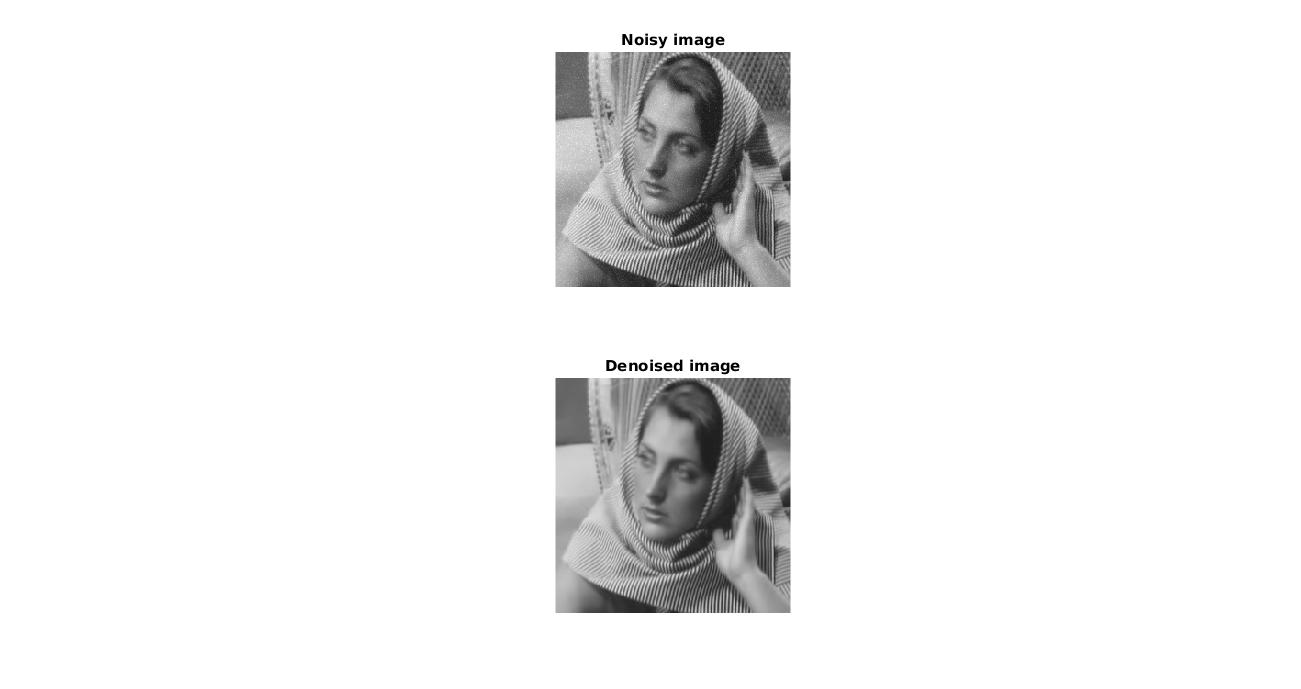
\includegraphics[scale=0.5]{q1a.jpg}
% 	\caption{Question 1a results}
% 	\label{Fig :1a}
% \end{figure}

% \begin{figure}[h]
%   % \centering
%   \begin{subfigure}[t]{0.32\textwidth}
%     \centering
%     \includegraphics[scale=0.5]{images/original_image_barbara}
%     \caption{Original Image Barbara}
%     \label{Fig :1a}
%   \end{subfigure}
%   ~
%   \begin{subfigure}[t]{0.32\textwidth}
%     \centering
%     \includegraphics[scale=0.5]{images/noisy_image_barbara}
%     \caption{Noisy Image Barbara}
%     \label{Fig :1b}
%   \end{subfigure}
%   ~
%   \begin{subfigure}[t]{0.32\textwidth}
%     \centering
%     \includegraphics[scale=0.5]{images/denoised_image_barbara}
%     \caption{Denoised Image Barbara}
%     \label{Fig: 1c}
%   \end{subfigure}

%   \caption{Figures for Q1}
% \end{figure}

\subsection*{A1.c}

The image corresponding to $ \Delta s = 0.5 $ pixel width unit is the smoothest because of the fact that due to a small step size the resolution of the obtained image is large as a result of subpixel accuracy and thus the image obtained is very smooth. \\
Again due to the same reason, the smaller value of $ \Delta s$ offers a a larger number of points due to smaller step size and hence we get a smoother plot.
% The code for this is question1b.m. The output is a little dark. Despite trying for different values of lambda and alpha the issue doesn't seem to get resolved.

% Parameters chosen:
% $$\lambda = 20$$
% $$\alpha = 1.01*\text{max}(\text{eig}(A'*A))$$

\begin{figure}[h]
	\centering
	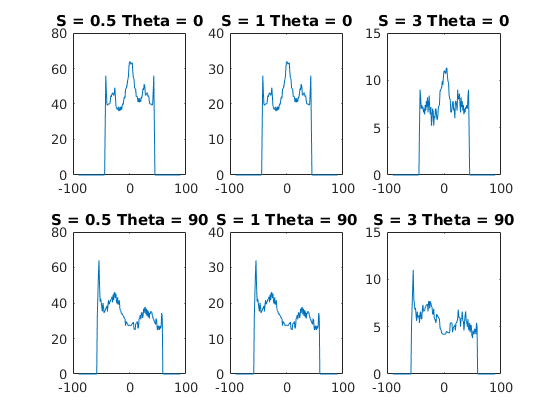
\includegraphics[scale = 0.7]{code/html/myRadonTrans_04.png}
	\caption{Plots}
	\label{Fig :1b}
\end{figure}

% \begin{figure}[h]
%   \begin{subfigure}[t]{0.5\textwidth}
%     \centering
%     \includegraphics[scale=0.5]{images/original_image_barbara}
%     \caption{Original Image Barbara}
%     \label{Fig :1a}
%   \end{subfigure}
%   ~
%   \begin{subfigure}[t]{0.5\textwidth}
%     \centering
%     \includegraphics[scale=0.5]{images/phi_reconstructed_barbara}
%     \caption{Reconstructed Image Barbara}
%     \label{Fig :1b}
%   \end{subfigure}
%   \caption{Figures for Q2}
% \end{figure}
\subsection*{A1.d}
The values of $ \Delta \theta $ used should be generally small in order to obtain a smooth image. We tried with different values of $ \Delta \theta $ and empirically obtained the result that a smaller value gives better results. However, it should not be very small because of the fact that since the system is discretized, a sub pixel update would not affect the value much and hence would not be very informative. Thus a reasonable value in the super pixel range must be taken. \\

The value of $ \Delta t $ has depends on the angles. For values close to $0$ or $90$ degrees, the a super pixel range incrememt would affect to a greater extent while somewhere in the middle of the range, sat $45$ degrees. However again due to discretizaton, a sub pixel increment in the middle region will not lead to a significant increase in the information. Thus the choice depends somewhat on the choice of $ \Delta \theta $ and also the size of the image. In a larger image a larger value can be supported without much problems. \\

Thus keeping in mind the above points we must choose the values of $ \Delta \theta $ and $ \Delta t $. \\

On plotting we found that the smaller values of $\Delta t $ gave good results naturally because it meant greater amount of information and hence better plot. However, as an expected consequence, the time taken was considerably larger. A similar pattern was obtained for a variation in $\Delta \theta$. For very small values, the obtained image is very smooth as shown in the figures below.

\begin{figure}[h]
	\centering
	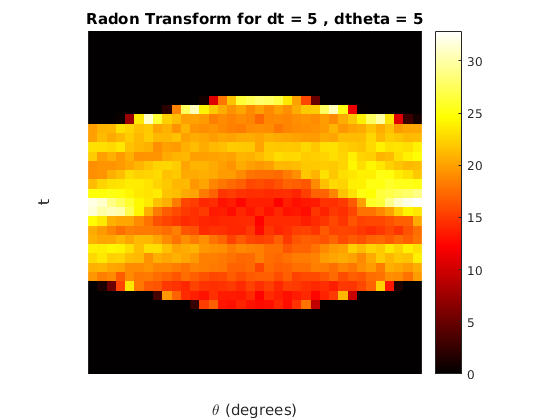
\includegraphics[scale = 0.5]{code/html/myRadonTrans_05.png}
	\caption{For $\Delta t = 5, \Delta \theta =5 $}
	\label{Fig :1d1}
\end{figure}

\begin{figure}[h]
	\centering
	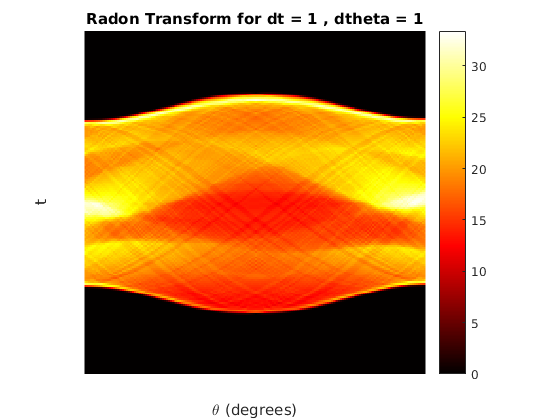
\includegraphics[scale = 0.5]{code/html/myRadonTrans_07.png}
	\caption{For $\Delta t = 1, \Delta \theta =1 $}
	\label{Fig :1d2}
\end{figure}
% In the folder q1, run the file deblur.m to get the deblurred image.

% The code for this is question1c.m. The code takes a parameter of the magnitude of the noise relative to the magnitude of the signal expressed in percentage.

\subsection*{A1.e}
As far as the number of pixels in the grid is considered, one of the major concerns is about the fact that larger the grid, more the time it takes to reconstruct the image. However, naturally, a larger image helps in having a greater degree of accuracy and hence better quality. \\

The effect of choosing $ \Delta s $ is reflected in the fact how smooth the final image looks like. A larger $ \Delta s $ implies taking large steps which means the reconstruction will happen at a scale larger than pixel width which would mean that finally to obtain the missing pixel values one would need to interpolate resulting a relatively rougher image. Consequently, a smaller value of $ \Delta s $ implies reconstruction at a sub pixel range which means that the image that is formed has a very high resolution and thus is very smooth and detailed. It might seem from the above comments that a natural choice for $ \Delta s $ is as small as possible, however, a smaller value comes at a cost. The smaller the value, the longer it takes to reconstruct the image. This is the tradeoff one has to face while choosing the $ \Delta s $. \\

Thus given the time availability and the quality requirements, one can choose an optimal $ \Delta s $  and the grid size keeping in mind the tradeoff.  


\section*{Q2}
\subsection*{A2.a}

Here are the results for different values of $L$. Clearly there are more artefacts in the case when no filter is applied as compared to the others in both the different values of $L$.  Also the image is little brighter in the case of cosine filter in both the cases and the circles in the center are more clearly visible as compared to the other ones. Also, we note that the two dark central ellipses do not show up very well in the case of Ram Lak and Shepp Logan filters for the case of $L = w_{\text{max}/2}$. That is to say there are some pixels of different intensities as noise in the two patches. However, this noise is reduced in the case of the cosine filter. But for the case of $L = w_{\text{max}}$ we note that these noisy elements aren't visible for any of the cases. A similar argument is true for the other constant patches. However, we also note that in both the cases the boundary has been clearly demarcated in all the filters.
 
\begin{figure}[h]
	\centering
	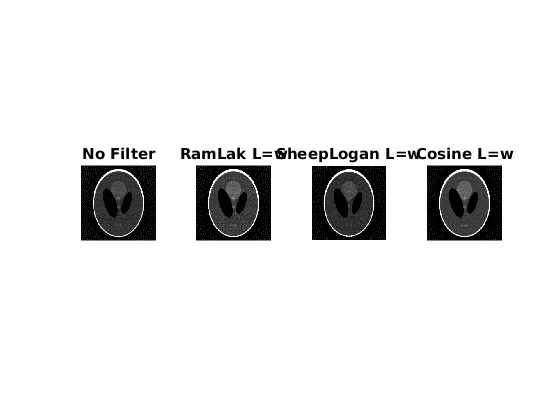
\includegraphics[scale = 0.9]{code/html/mainScript_02.png}
	\caption{For $L = w_{\text{max}}$}
	\label{Fig :2a1}
\end{figure}

\begin{figure}[h]
	\centering
	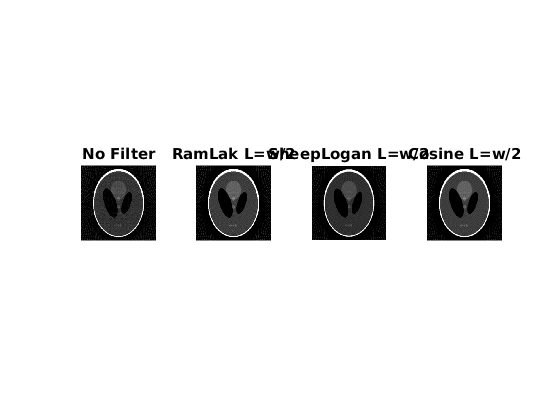
\includegraphics[scale = 0.9]{code/html/mainScript_03.png}
	\caption{$L = w_{\text{max}}/2$}
	\label{Fig :2a2}
\end{figure}

\subsection*{A2.b}

The issue with backprojection is the fact that due to the higher frequency components, we observe blurring in the projected image. And this increases with the increase in the magnitude of the higher frequency components. However, on blurring these components get reduced and we see that with the increase in the variance of the blur we obtain a greater reduction in the magnitude of the higher frequency components. As a result of which the image gets sharper and better as the blurring is increased. This is in accordance with the results obtained experimentally. This can be verified using the plot given below. It shows values for different values of blurring and it is clearly evident that on increasing the blur, the RMSE is reduced.

\subsection*{A2.c}

As the value of $L$ is increased the cutoff frequency of the filters is increased. An increase in the cutoff frequencies implies that the higher frequency components are boosted much more, which helps in betterment of the resconstructed image. This is clearly evident in the plot given below.

\begin{figure}[h]
	\centering
	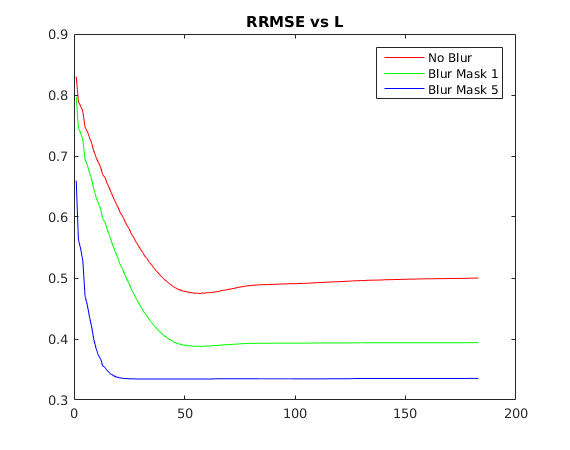
\includegraphics[scale = 0.8]{code/html/mainScript_08.png}
	\caption{RMSE vs L}
	\label{Fig :2c}
\end{figure}

As it can be seen from the plot the on increasing the value of $L$ there is a reduction in the value of RMSE. 


\end{document}

